\subsection{Feature Extraction}
    Excluding the label for each activity, each session in the dataset contains 589 features. These features were extracted by applying a number of different statistical
    measures to the different extracted signals in each sliding window.

    Each signal has the statistical measures in Table 1 applied to them.

    \begin{table}[ht]
        \begin{tabular}{|l|l|lll}
            \cline{1-2}
            \textbf{Statistical Measure} & \textbf{Description} &  &  &  \\ \cline{1-2}
            mean             & Mean value in the window           &  &  &  \\ \cline{1-2}
            min            & Smallest value in the window           &  &  &  \\ \cline{1-2}
            max            & Largest value in the window           &  &  & \\ \cline{1-2}
            std            & Standard deviation           &  &  & \\ \cline{1-2}
            entropy            & Entropy           &  &  & \\ \cline{1-2}
            mad            & 3           &  &  & \\ \cline{1-2}
            iqr            & Inter-quartile Range           &  &  & \\ \cline{1-2}
            energy            & 3           &  &  & \\ \cline{1-2}
            sma            & Signal magnitude area           &  &  & \\ \cline{1-2}
            arCoeff            & 3           &  &  & \\ \cline{1-2}
            correlation            & 3           &  &  & \\ \cline{1-2}
            angle            & Angle between 2 vectors of signals           &  &  & \\ \cline{1-2}
            band energy            & 3           &  &  & \\ \cline{1-2}
        \end{tabular}
        \caption*{Table 1}
    \end{table}

    The statistical measures in Table 2 are applied only to FFT signals.

    \begin{table}[ht]
        \begin{tabular}{|l|l|lll}
            \cline{1-2}
            \textbf{Statistical Measure} & \textbf{Description} &  &  &  \\ \cline{1-2}
            maxInds             & 1           &  &  &  \\ \cline{1-2}
            skewness            & 2           &  &  &  \\ \cline{1-2}
            kurtosis               & 3           &  &  &  \\ \cline{1-2}
            meanFreq            & 3           &  &  &  \\ \cline{1-2}
        \end{tabular}
        \caption*{Table 2}
    \end{table}


\subsection{Signal Processing}

\subsection{Support Vector Classifier}
    \subsubsection{Data Pre-processing}
        Firstly, the training and testing datasets were converted to Pandas dataframes and the labels for each activity were separated into their own variables.
        Using a LabelEncoder, each activity label is converted into a numerical value.

    \subsubsection{Comparing different classification models}
        In total, four different classic machine learning classifiers were used on the dataset developed by Anguita et al \cite{Anguita2012}. These classifiers are Gaussian Naïve Bayes,
        AdaBoost, Stochastic Gradient Descent and a Support Vector Classifier. These were trained and tested using the respective datasets, and their accuracy,
        F-beta, precision and recall scores were recorded.

        \begin{table}[ht]
            \centering\footnotesize
            \begin{tabular}{|l|l|l|l|l|}
                \hline
                \textbf{Classifier} & \textbf{Accuracy} & \textbf{F-Beta}  & \textbf{Precision} & \textbf{Recall} \\ \hline
                Gaussian Naïve Bayes             & 0.7134           & 0.7252  & 0.7555 & 0.7134 \\ \hline
                AdaBoost            & 0.4065           & 0.2520 & 0.4289 & 0.4065 \\ \hline
                Stochastic Gradient Descent               & 0.9600           & 0.9603 & 0.9605 & 0.9600 \\ \hline
                Support Vector Classifier            & 0.9668           & 0.9676 & 0.9682 & 0.9668 \\ \hline
            \end{tabular}
            \caption*{Table 3: Performance scores of each classifier}
        \end{table}

        As can be seen in Table 3, the Support Vector Classifier had the highest scores, each result being over 0.96. It is for this reason that the SVC
        was chosen to classify the UCI dataset \cite{Anguita2013} and, later on, the dataset built by ourselves.

    \subsection{Classification}
        The RBF kernel is defined as the exponential function \(exp(-\gamma \lvert x-x' \rvert)^2\) A primer on kernel methods, JP Vert et al, where x and x’ are two feature vectors, and is the
        gamma parameter in the classifier. Gamma’s value is scale, meaning that the parameter is the reciprocal of the number of features multiplied with the variance of the input data.
        For this implementation, we opted for a One-Vs-All approach. A One-Vs-All approach divides the data points into just two classes: a certain activity X and the other classes. Therefore records
        labelled as \emph{SITTING} are a single class, and the other activities are treated as having a single label.

\subsection{Convolutional Neural Networks}
    In the research done numerous CNN implementations designed for the UCI dataset like [include numerous] were checked.
    From these, [paper] presented the choice and implementation of a CNN use for HAR the best.
    Hence, the implementation described in this report is based on the architectures described in [the paper].
    Unlike [paper authors] we did not  implement a first stage dynamic-static split model and instead opted to split the labels manually.
    The Pytorch [reference it] library was used to implement the CNNs, and the sklearn [reference it] library to evaluate the results.

    \subsubsection{Data Split}
        The train/valid/test split was an 80/20 train/test split, then 80/20 train/validation split for the UCI dataset, and a 90/10 train/test split, then 90/10 train/validation split for Our Dataset.
    \subsubsection{Dataset Object}
        To facilitate this dynamic/static split we defined a Python dictionary with each label having a number assigned to it, starting from 0.
        The numbering needs to start from 0 as the output of neural networks implemented in Pytorch always start from 0.
        Another requirement for implementing neural networks in Pytorch is to implement a custom Dataset object.
        The function of this object is to read the data from a source and define its X, data and Y, labels counterparts.
        The Pandas [reference it] library was used at this stage due to its use of the numpy [reference it] library and efficient data management.
        It is important that the X component is in the shape: length(data.columns), 1, length(data.rows)).

        The dataset object was initialised 3 times, for the Train, Validation and Testing data.

        The pie charts included below show the training, validation and testing label distribution in order.

        \begin{figure}[h]
        \centering
        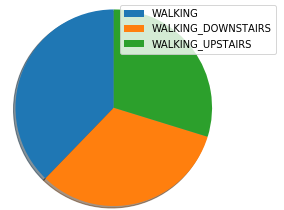
\includegraphics[width=.15\textwidth]{UCI_Dynamic_Training}\hfill
        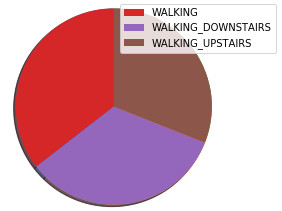
\includegraphics[width=.15\textwidth]{UCI_Dynamic_Validation}\hfill
        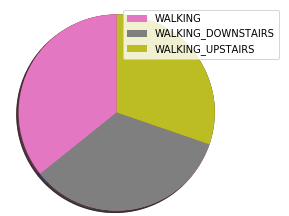
\includegraphics[width=.15\textwidth]{UCI_Dynamic_Testing}
        \caption{UCI Dynamic Label Distribution}
        \label{fig:figureX}
        \end{figure}

        \begin{figure}[h]
        \centering
        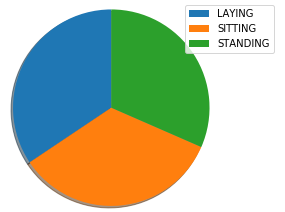
\includegraphics[width=.15\textwidth]{UCI_Static_Training}\hfill
        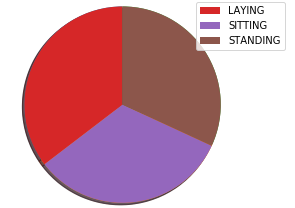
\includegraphics[width=.15\textwidth]{UCI_Static_Validation}\hfill
        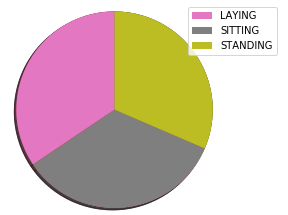
\includegraphics[width=.15\textwidth]{UCI_Static_Testing}
        \caption{UCI Static Label Distribution}
        \label{fig:figureX}
        \end{figure}

        \begin{figure}[h]
        \centering
        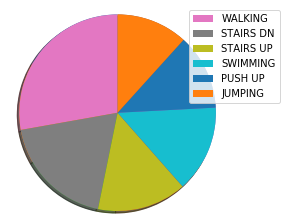
\includegraphics[width=.15\textwidth]{OD_Dynamic_Training}\hfill
        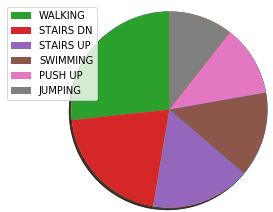
\includegraphics[width=.15\textwidth]{OD_Dynamic_Validation}\hfill
        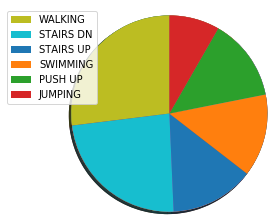
\includegraphics[width=.15\textwidth]{OD_Dynamic_Testing}
        \caption{OD Dynamic Label Distribution}
        \label{fig:figureX}
        \end{figure}

        \begin{figure}[h]
        \centering
        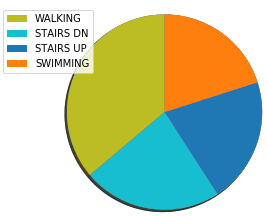
\includegraphics[width=.15\textwidth]{OD_Static_Training}\hfill
        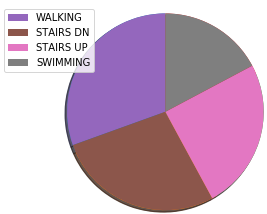
\includegraphics[width=.15\textwidth]{OD_Static_Validation}\hfill
        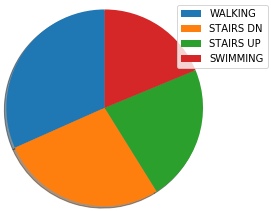
\includegraphics[width=.15\textwidth]{OD_Static_Testing}
        \caption{OD Static Label Distribution}
        \label{fig:figureX}
        \end{figure}

        In development, it was noted that the data distribution of the dynamic activities in our dataset was unequal.
        This was causing issues with the CNN's accuracy.
        To combat this added functionality was added with the aim of increase the quality of the model's output.
        In this project the number of rows for each eligible label was stored.
        Using the functionality provided by the Pandas library, the index for each label was stored in a list linked to its respective label.
        Using Python list slicing these lists where cut down to their lowest common length.
        These indices where then converted into a new Pandas dataframe and this balanced dataset was used for the dynamic model.

        \begin{figure}[h]
        \centering
        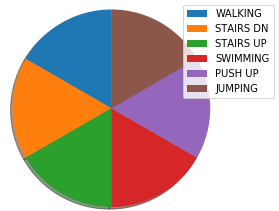
\includegraphics[width=.15\textwidth]{OD_Dynamic_Training_Balanced}\hfill
        \caption{OD Dynamic Training Balanced Label Distribution}
        \label{fig:figureX}
        \end{figure}

        Finally the dataset objects are used to initialise a Dataloader object.
        This object gives us the functionality of delivering batches as inputs to the models at training and testing.
        It was found that a batch size of 32 worked best for the Static models, and a batch size of 64 worked best for the dynamic models.

    \subsubsection{Model Creation}
        The CNN models where implemented following the design of the below diagrams.
        Every model used the Cross Entropy as their loss function and the ADAM optimizer.
        The learning rate for the UCI Dataset Models, and Our Dataset Static model was set at 0.0005 and were trained for 10 epochs.
        The learning rate for the Our Dataset Dynamic model was set at 0.00005 and were trained for 11 epochs.

        \begin{figure}[h]
        \centering
        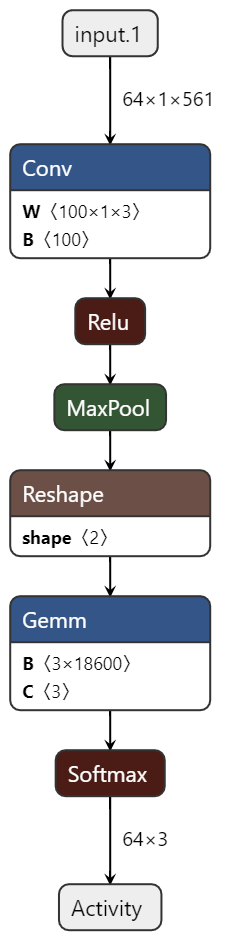
\includegraphics[width=.15\textwidth]{DCNN}\hfill
        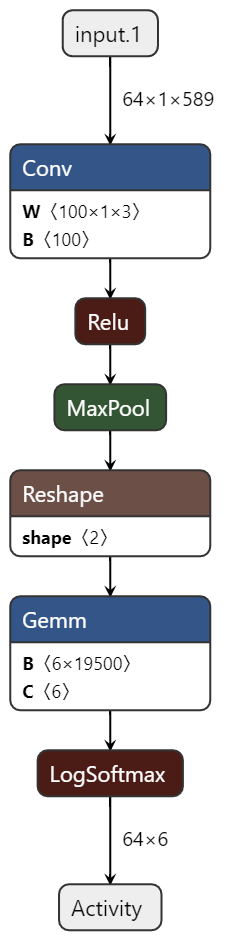
\includegraphics[width=.15\textwidth]{ODDCNN}\hfill
        \caption{UCI(left) and OD(right) Dynamic Model Structure}
        \label{fig:figureX}
        \end{figure}

        \begin{figure}[h]
        \centering
        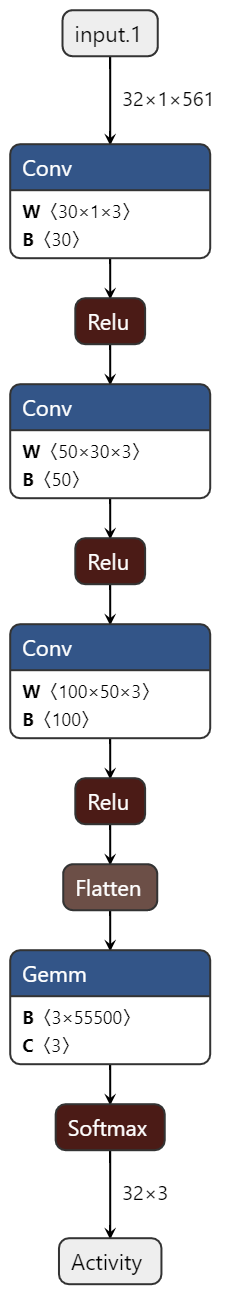
\includegraphics[width=.15\textwidth]{SCNN}\hfill
        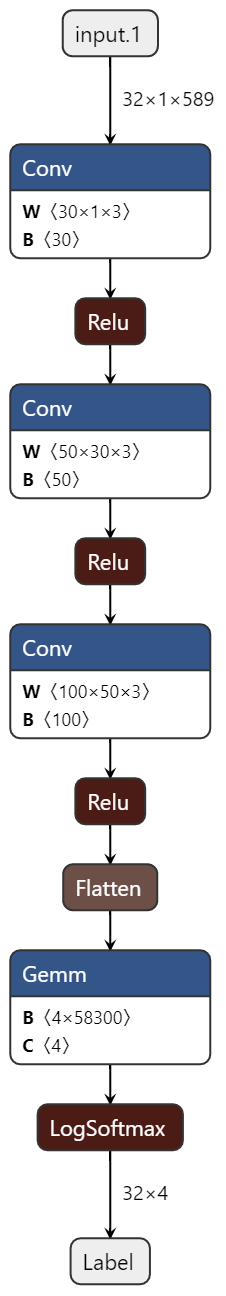
\includegraphics[width=.15\textwidth]{ODSCNN}\hfill
        \caption{UCI(left) and OD(right) Static Model Structure}
        \label{fig:figureX}
        \end{figure}

        As seen in figures X and X the four models follow the a similar structure having a Convolutional layer that is then followed by a fully connected layer.
        The OD models differentiate at the final activation function where it was found that the Softmax activation function was not activating properly.
        Seeing this another activation function was used, the LogSoftmax function.
        It is also worthwhile to note that the final layer fully connected layer is different since the UCI dataset and Our dataset have a different number of total features.
